\section{Audio clipping}

\begin{figure}[H]
\centering
\begin{subfigure}[b]{0.47\textwidth}
	\tikzsetnextfilename{clippingClean}
	% This file was created by matlab2tikz.
%
%The latest updates can be retrieved from
%  http://www.mathworks.com/matlabcentral/fileexchange/22022-matlab2tikz-matlab2tikz
%where you can also make suggestions and rate matlab2tikz.
%
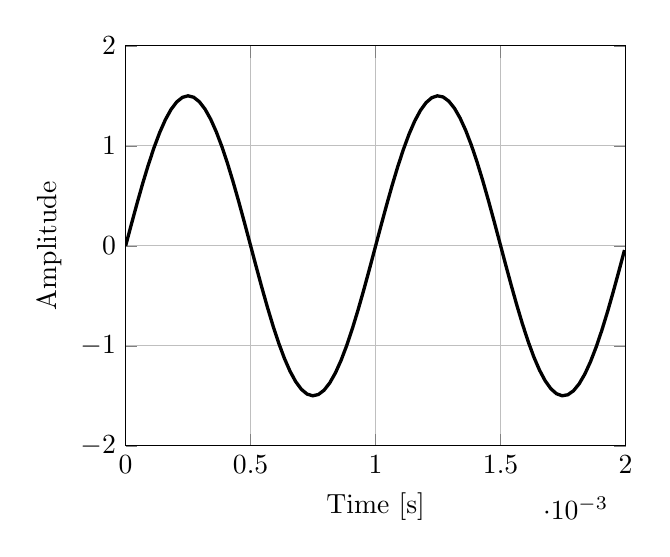
\begin{tikzpicture}

\begin{axis}[%
width=2.5in,
height=2in,
at={(1.011in,0.642in)},
scale only axis,
xmin=0,
xmax=0.002,
xlabel={Time [s]},
xmajorgrids,
ymin=-2,
ymax=2,
ylabel={Amplitude},
ymajorgrids,
axis background/.style={fill=white}
]
\addplot [color=black,solid,line width=1.2pt,forget plot]
  table[row sep=crcr]{%
0	0\\
2.26757369614512e-05	0.21299147693644\\
4.53514739229025e-05	0.421666669997482\\
6.80272108843537e-05	0.621796765035443\\
9.0702947845805e-05	0.809326114779272\\
0.000113378684807256	0.98045442674729\\
0.000136054421768707	1.13171377638122\\
0.000158730158730159	1.26003888472616\\
0.00018140589569161	1.36282923647545\\
0.000204081632653061	1.43800177955499\\
0.000226757369614512	1.48403313828686\\
0.000249433106575964	1.49999048468041\\
0.000272108843537415	1.48555044224226\\
0.000294784580498866	1.44100563921852\\
0.000317460317460317	1.36725877846751\\
0.000340136054421769	1.26580434413712\\
0.00036281179138322	1.13869831586227\\
0.000385487528344671	0.988516504225587\\
0.000408163265306122	0.818302351815823\\
0.000430839002267574	0.631505257698036\\
0.000453514739229025	0.431910675153779\\
0.000476190476190476	0.223563399264262\\
0.000498866213151927	0.0106855989178377\\
0.000521541950113379	-0.202408745672383\\
0.00054421768707483	-0.411401266012395\\
0.000566893424036281	-0.612056717299934\\
0.000589569160997732	-0.800308805890951\\
0.000612244897959184	-0.972342592961682\\
0.000634920634920635	-1.1246718044516\\
0.000657596371882086	-1.25420948059704\\
0.000680272108843537	-1.35833053333888\\
0.000702947845804989	-1.43492494387492\\
0.00072562358276644	-1.48244052230586\\
0.000748299319727891	-1.49991436284804\\
0.000770975056689342	-1.48699235717159\\
0.000793650793650794	-1.44393637042502\\
0.000816326530612245	-1.37161893452372\\
0.000839002267573696	-1.2715055662432\\
0.000861678004535147	-1.14562506844185\\
0.000884353741496599	-0.996528416260569\\
0.00090702947845805	-0.827237061472641\\
0.000929705215419501	-0.641181702599088\\
0.000952380952380952	-0.442132761616357\\
0.000975056689342404	-0.234123976149712\\
0.000997732426303855	-0.0213706555606557\\
0.00102040816326531	0.191815742526759\\
0.00104308390022676	0.401114984149397\\
0.00106575963718821	0.602285608781499\\
0.00108843537414966	0.791250882763146\\
0.00111111111111111	0.964181414529808\\
0.00113378684807256	1.11757275744087\\
0.00115646258503401	1.24831642758161\\
0.00117913832199546	1.35376289735891\\
0.00120181405895692	1.43177528832223\\
0.00122448979591837	1.48077267512167\\
0.00124716553287982	1.49976212304635\\
0.00126984126984127	1.48835880990026\\
0.00129251700680272	1.44679382444511\\
0.00131519274376417	1.37590948337396\\
0.00133786848072562	1.27714226171757\\
0.00136054421768707	1.15249368259969\\
0.00138321995464853	1.00448975626204\\
0.00140589569160998	0.836129790329203\\
0.00142857142857143	0.650825608676338\\
0.00145124716553288	0.452332410632626\\
0.00147392290249433	0.244672671662413\\
0.00149659863945578	0.0320546276809519\\
0.00151927437641723	-0.181213005075519\\
0.00154195011337868	-0.390808346418877\\
0.00156462585034014	-0.592483935346407\\
0.00158730158730159	-0.782152805069245\\
0.00160997732426304	-0.955971305616867\\
0.00163265306122449	-1.11041699561297\\
0.00165532879818594	-1.24236002474175\\
0.00167800453514739	-1.34912656033491\\
0.00170068027210884	-1.42855297273628\\
0.00172335600907029	-1.47902968137455\\
0.00174603174603175	-1.49953377300122\\
0.0017687074829932	-1.48964973108323\\
0.00179138321995465	-1.44957785626813\\
0.0018140589569161	-1.38013020728057\\
0.00183673469387755	-1.28271414450802\\
0.001859410430839	-1.15930380976591\\
0.00188208616780045	-1.01240012020625\\
0.0019047619047619	-0.844980087095434\\
0.00192743764172336	-0.660436486518814\\
0.00195011337868481	-0.462509104588652\\
0.00197278911564626	-0.25520895047495\\
0.00199546485260771	-0.0427369730862695\\
};
\end{axis}
\end{tikzpicture}%
	\caption{Test.}
	\label{fig:clippingClean}
\end{subfigure}
\hspace{6mm} 
\begin{subfigure}[b]{0.47\textwidth}
	\tikzsetnextfilename{clippingDist}
	% This file was created by matlab2tikz.
%
%The latest updates can be retrieved from
%  http://www.mathworks.com/matlabcentral/fileexchange/22022-matlab2tikz-matlab2tikz
%where you can also make suggestions and rate matlab2tikz.
%
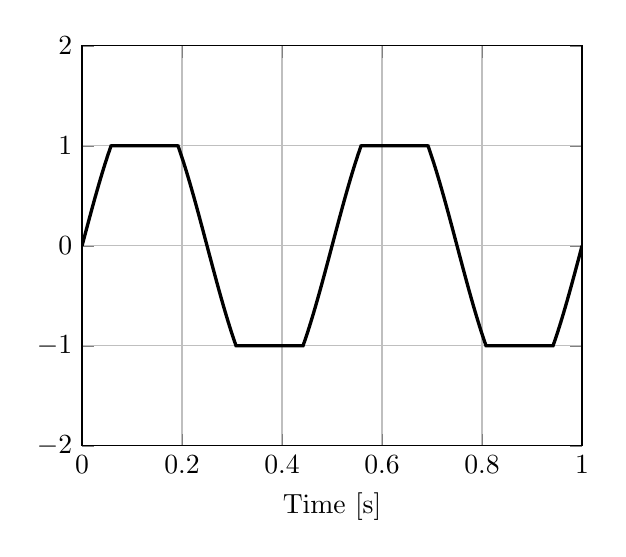
\begin{tikzpicture}

\begin{axis}[%
width=2.5in,
height=2in,
at={(1.011in,0.642in)},
scale only axis,
xmin=0,
xmax=1,
xlabel={Time [s]},
xmajorgrids,
ymin=-2,
ymax=2,
ymajorgrids,
axis background/.style={fill=white}
]
\addplot [color=black,solid,line width=1.2pt,forget plot]
  table[row sep=crcr]{%
0	0\\
0.001	0.0188490598250289\\
0.002	0.0376951431650062\\
0.003	0.0565352740049018\\
0.004	0.0753664772696543\\
0.005	0.0941857792939701\\
0.006	0.112990208291899\\
0.007	0.131776794826115\\
0.008	0.150542572276822\\
0.009	0.169284577310223\\
0.01	0.187999850346456\\
0.011	0.206685436026957\\
0.012	0.225338383681136\\
0.013	0.243955747792325\\
0.014	0.262534588462914\\
0.015	0.281071971878587\\
0.016	0.299564970771611\\
0.017	0.318010664883082\\
0.018	0.336406141424072\\
0.019	0.354748495535587\\
0.02	0.373034830747282\\
0.021	0.391262259434845\\
0.022	0.409427903275988\\
0.023	0.427528893704964\\
0.024	0.445562372365552\\
0.025	0.463525491562421\\
0.026	0.481415414710814\\
0.027	0.49922931678448\\
0.028	0.516964384761776\\
0.029	0.534617818069876\\
0.03	0.552186829027017\\
0.031	0.569668643282702\\
0.032	0.587060500255804\\
0.033	0.604359653570494\\
0.034	0.621563371489926\\
0.035	0.638668937347609\\
0.036	0.655673649976399\\
0.037	0.672574824135048\\
0.038	0.689369790932232\\
0.039	0.706055898247999\\
0.04	0.722630511152573\\
0.041	0.739091012322437\\
0.042	0.755434802453641\\
0.043	0.77165930067226\\
0.044	0.787761944941943\\
0.045	0.803740192468495\\
0.046	0.819591520101404\\
0.047	0.835313424732282\\
0.048	0.850903423690135\\
0.049	0.866359055133401\\
0.05	0.88167787843871\\
0.051	0.896857474586278\\
0.052	0.911895446541908\\
0.053	0.926789419635502\\
0.054	0.941537041936051\\
0.055	0.956135984623034\\
0.056	0.970583942354166\\
0.057	0.984878633629435\\
0.058	0.999017801151378\\
0.059	1\\
0.06	1\\
0.061	1\\
0.062	1\\
0.063	1\\
0.064	1\\
0.065	1\\
0.066	1\\
0.067	1\\
0.068	1\\
0.069	1\\
0.07	1\\
0.071	1\\
0.072	1\\
0.073	1\\
0.074	1\\
0.075	1\\
0.076	1\\
0.077	1\\
0.078	1\\
0.079	1\\
0.08	1\\
0.081	1\\
0.082	1\\
0.083	1\\
0.084	1\\
0.085	1\\
0.086	1\\
0.087	1\\
0.088	1\\
0.089	1\\
0.09	1\\
0.091	1\\
0.092	1\\
0.093	1\\
0.094	1\\
0.095	1\\
0.096	1\\
0.097	1\\
0.098	1\\
0.099	1\\
0.1	1\\
0.101	1\\
0.102	1\\
0.103	1\\
0.104	1\\
0.105	1\\
0.106	1\\
0.107	1\\
0.108	1\\
0.109	1\\
0.11	1\\
0.111	1\\
0.112	1\\
0.113	1\\
0.114	1\\
0.115	1\\
0.116	1\\
0.117	1\\
0.118	1\\
0.119	1\\
0.12	1\\
0.121	1\\
0.122	1\\
0.123	1\\
0.124	1\\
0.125	1\\
0.126	1\\
0.127	1\\
0.128	1\\
0.129	1\\
0.13	1\\
0.131	1\\
0.132	1\\
0.133	1\\
0.134	1\\
0.135	1\\
0.136	1\\
0.137	1\\
0.138	1\\
0.139	1\\
0.14	1\\
0.141	1\\
0.142	1\\
0.143	1\\
0.144	1\\
0.145	1\\
0.146	1\\
0.147	1\\
0.148	1\\
0.149	1\\
0.15	1\\
0.151	1\\
0.152	1\\
0.153	1\\
0.154	1\\
0.155	1\\
0.156	1\\
0.157	1\\
0.158	1\\
0.159	1\\
0.16	1\\
0.161	1\\
0.162	1\\
0.163	1\\
0.164	1\\
0.165	1\\
0.166	1\\
0.167	1\\
0.168	1\\
0.169	1\\
0.17	1\\
0.171	1\\
0.172	1\\
0.173	1\\
0.174	1\\
0.175	1\\
0.176	1\\
0.177	1\\
0.178	1\\
0.179	1\\
0.18	1\\
0.181	1\\
0.182	1\\
0.183	1\\
0.184	1\\
0.185	1\\
0.186	1\\
0.187	1\\
0.188	1\\
0.189	1\\
0.19	1\\
0.191	1\\
0.192	0.999017801151378\\
0.193	0.984878633629435\\
0.194	0.970583942354166\\
0.195	0.956135984623035\\
0.196	0.941537041936051\\
0.197	0.926789419635502\\
0.198	0.911895446541908\\
0.199	0.896857474586278\\
0.2	0.88167787843871\\
0.201	0.866359055133402\\
0.202	0.850903423690135\\
0.203	0.835313424732282\\
0.204	0.819591520101404\\
0.205	0.803740192468495\\
0.206	0.787761944941943\\
0.207	0.771659300672259\\
0.208	0.755434802453641\\
0.209	0.739091012322437\\
0.21	0.722630511152573\\
0.211	0.706055898247999\\
0.212	0.689369790932232\\
0.213	0.672574824135048\\
0.214	0.655673649976399\\
0.215	0.638668937347609\\
0.216	0.621563371489926\\
0.217	0.604359653570494\\
0.218	0.587060500255804\\
0.219	0.569668643282702\\
0.22	0.552186829027017\\
0.221	0.534617818069876\\
0.222	0.516964384761776\\
0.223	0.49922931678448\\
0.224	0.481415414710815\\
0.225	0.463525491562421\\
0.226	0.445562372365552\\
0.227	0.427528893704964\\
0.228	0.409427903275988\\
0.229	0.391262259434846\\
0.23	0.373034830747282\\
0.231	0.354748495535587\\
0.232	0.336406141424071\\
0.233	0.318010664883082\\
0.234	0.299564970771611\\
0.235	0.281071971878587\\
0.236	0.262534588462914\\
0.237	0.243955747792325\\
0.238	0.225338383681136\\
0.239	0.206685436026957\\
0.24	0.187999850346457\\
0.241	0.169284577310223\\
0.242	0.150542572276822\\
0.243	0.131776794826115\\
0.244	0.1129902082919\\
0.245	0.0941857792939704\\
0.246	0.0753664772696545\\
0.247	0.0565352740049018\\
0.248	0.0376951431650067\\
0.249	0.0188490598250293\\
0.25	1.83697019872103e-16\\
0.251	-0.0188490598250289\\
0.252	-0.0376951431650064\\
0.253	-0.0565352740049014\\
0.254	-0.0753664772696541\\
0.255	-0.09418577929397\\
0.256	-0.112990208291899\\
0.257	-0.131776794826114\\
0.258	-0.150542572276822\\
0.259	-0.169284577310222\\
0.26	-0.187999850346456\\
0.261	-0.206685436026957\\
0.262	-0.225338383681135\\
0.263	-0.243955747792325\\
0.264	-0.262534588462914\\
0.265	-0.281071971878587\\
0.266	-0.299564970771611\\
0.267	-0.318010664883082\\
0.268	-0.336406141424072\\
0.269	-0.354748495535587\\
0.27	-0.373034830747282\\
0.271	-0.391262259434845\\
0.272	-0.409427903275988\\
0.273	-0.427528893704964\\
0.274	-0.445562372365553\\
0.275	-0.463525491562422\\
0.276	-0.481415414710814\\
0.277	-0.49922931678448\\
0.278	-0.516964384761776\\
0.279	-0.534617818069876\\
0.28	-0.552186829027017\\
0.281	-0.569668643282702\\
0.282	-0.587060500255804\\
0.283	-0.604359653570494\\
0.284	-0.621563371489927\\
0.285	-0.638668937347609\\
0.286	-0.6556736499764\\
0.287	-0.672574824135049\\
0.288	-0.689369790932232\\
0.289	-0.706055898247998\\
0.29	-0.722630511152572\\
0.291	-0.739091012322437\\
0.292	-0.755434802453641\\
0.293	-0.771659300672259\\
0.294	-0.787761944941943\\
0.295	-0.803740192468495\\
0.296	-0.819591520101403\\
0.297	-0.835313424732281\\
0.298	-0.850903423690134\\
0.299	-0.866359055133401\\
0.3	-0.88167787843871\\
0.301	-0.896857474586278\\
0.302	-0.911895446541908\\
0.303	-0.926789419635501\\
0.304	-0.94153704193605\\
0.305	-0.956135984623034\\
0.306	-0.970583942354166\\
0.307	-0.984878633629434\\
0.308	-0.999017801151377\\
0.309	-1\\
0.31	-1\\
0.311	-1\\
0.312	-1\\
0.313	-1\\
0.314	-1\\
0.315	-1\\
0.316	-1\\
0.317	-1\\
0.318	-1\\
0.319	-1\\
0.32	-1\\
0.321	-1\\
0.322	-1\\
0.323	-1\\
0.324	-1\\
0.325	-1\\
0.326	-1\\
0.327	-1\\
0.328	-1\\
0.329	-1\\
0.33	-1\\
0.331	-1\\
0.332	-1\\
0.333	-1\\
0.334	-1\\
0.335	-1\\
0.336	-1\\
0.337	-1\\
0.338	-1\\
0.339	-1\\
0.34	-1\\
0.341	-1\\
0.342	-1\\
0.343	-1\\
0.344	-1\\
0.345	-1\\
0.346	-1\\
0.347	-1\\
0.348	-1\\
0.349	-1\\
0.35	-1\\
0.351	-1\\
0.352	-1\\
0.353	-1\\
0.354	-1\\
0.355	-1\\
0.356	-1\\
0.357	-1\\
0.358	-1\\
0.359	-1\\
0.36	-1\\
0.361	-1\\
0.362	-1\\
0.363	-1\\
0.364	-1\\
0.365	-1\\
0.366	-1\\
0.367	-1\\
0.368	-1\\
0.369	-1\\
0.37	-1\\
0.371	-1\\
0.372	-1\\
0.373	-1\\
0.374	-1\\
0.375	-1\\
0.376	-1\\
0.377	-1\\
0.378	-1\\
0.379	-1\\
0.38	-1\\
0.381	-1\\
0.382	-1\\
0.383	-1\\
0.384	-1\\
0.385	-1\\
0.386	-1\\
0.387	-1\\
0.388	-1\\
0.389	-1\\
0.39	-1\\
0.391	-1\\
0.392	-1\\
0.393	-1\\
0.394	-1\\
0.395	-1\\
0.396	-1\\
0.397	-1\\
0.398	-1\\
0.399	-1\\
0.4	-1\\
0.401	-1\\
0.402	-1\\
0.403	-1\\
0.404	-1\\
0.405	-1\\
0.406	-1\\
0.407	-1\\
0.408	-1\\
0.409	-1\\
0.41	-1\\
0.411	-1\\
0.412	-1\\
0.413	-1\\
0.414	-1\\
0.415	-1\\
0.416	-1\\
0.417	-1\\
0.418	-1\\
0.419	-1\\
0.42	-1\\
0.421	-1\\
0.422	-1\\
0.423	-1\\
0.424	-1\\
0.425	-1\\
0.426	-1\\
0.427	-1\\
0.428	-1\\
0.429	-1\\
0.43	-1\\
0.431	-1\\
0.432	-1\\
0.433	-1\\
0.434	-1\\
0.435	-1\\
0.436	-1\\
0.437	-1\\
0.438	-1\\
0.439	-1\\
0.44	-1\\
0.441	-1\\
0.442	-0.999017801151378\\
0.443	-0.984878633629435\\
0.444	-0.970583942354166\\
0.445	-0.956135984623034\\
0.446	-0.94153704193605\\
0.447	-0.926789419635502\\
0.448	-0.911895446541909\\
0.449	-0.896857474586279\\
0.45	-0.88167787843871\\
0.451	-0.866359055133402\\
0.452	-0.850903423690135\\
0.453	-0.835313424732282\\
0.454	-0.819591520101403\\
0.455	-0.803740192468494\\
0.456	-0.787761944941943\\
0.457	-0.77165930067226\\
0.458	-0.755434802453641\\
0.459	-0.739091012322437\\
0.46	-0.722630511152573\\
0.461	-0.706055898247999\\
0.462	-0.689369790932232\\
0.463	-0.672574824135048\\
0.464	-0.655673649976399\\
0.465	-0.638668937347608\\
0.466	-0.621563371489927\\
0.467	-0.604359653570494\\
0.468	-0.587060500255804\\
0.469	-0.569668643282702\\
0.47	-0.552186829027017\\
0.471	-0.534617818069876\\
0.472	-0.516964384761775\\
0.473	-0.499229316784479\\
0.474	-0.481415414710814\\
0.475	-0.463525491562421\\
0.476	-0.445562372365553\\
0.477	-0.427528893704964\\
0.478	-0.409427903275988\\
0.479	-0.391262259434845\\
0.48	-0.373034830747283\\
0.481	-0.354748495535588\\
0.482	-0.336406141424072\\
0.483	-0.318010664883082\\
0.484	-0.299564970771611\\
0.485	-0.281071971878587\\
0.486	-0.262534588462914\\
0.487	-0.243955747792326\\
0.488	-0.225338383681137\\
0.489	-0.206685436026958\\
0.49	-0.187999850346457\\
0.491	-0.169284577310223\\
0.492	-0.150542572276823\\
0.493	-0.131776794826115\\
0.494	-0.112990208291899\\
0.495	-0.0941857792939699\\
0.496	-0.0753664772696553\\
0.497	-0.0565352740049027\\
0.498	-0.0376951431650069\\
0.499	-0.0188490598250294\\
0.5	-3.67394039744206e-16\\
0.501	0.0188490598250287\\
0.502	0.0376951431650062\\
0.503	0.0565352740049019\\
0.504	0.0753664772696546\\
0.505	0.0941857792939692\\
0.506	0.112990208291898\\
0.507	0.131776794826114\\
0.508	0.150542572276822\\
0.509	0.169284577310222\\
0.51	0.187999850346456\\
0.511	0.206685436026957\\
0.512	0.225338383681136\\
0.513	0.243955747792326\\
0.514	0.262534588462913\\
0.515	0.281071971878586\\
0.516	0.29956497077161\\
0.517	0.318010664883082\\
0.518	0.336406141424072\\
0.519	0.354748495535587\\
0.52	0.373034830747282\\
0.521	0.391262259434843\\
0.522	0.409427903275988\\
0.523	0.427528893704962\\
0.524	0.445562372365552\\
0.525	0.46352549156242\\
0.526	0.481415414710814\\
0.527	0.499229316784479\\
0.528	0.516964384761776\\
0.529	0.534617818069874\\
0.53	0.552186829027017\\
0.531	0.5696686432827\\
0.532	0.587060500255804\\
0.533	0.604359653570492\\
0.534	0.621563371489926\\
0.535	0.638668937347608\\
0.536	0.655673649976399\\
0.537	0.672574824135046\\
0.538	0.689369790932232\\
0.539	0.706055898247997\\
0.54	0.722630511152573\\
0.541	0.739091012322436\\
0.542	0.755434802453641\\
0.543	0.771659300672258\\
0.544	0.787761944941944\\
0.545	0.803740192468494\\
0.546	0.819591520101404\\
0.547	0.83531342473228\\
0.548	0.850903423690135\\
0.549	0.8663590551334\\
0.55	0.88167787843871\\
0.551	0.896857474586277\\
0.552	0.911895446541908\\
0.553	0.9267894196355\\
0.554	0.941537041936051\\
0.555	0.956135984623034\\
0.556	0.970583942354167\\
0.557	0.984878633629433\\
0.558	0.999017801151378\\
0.559	1\\
0.56	1\\
0.561	1\\
0.562	1\\
0.563	1\\
0.564	1\\
0.565	1\\
0.566	1\\
0.567	1\\
0.568	1\\
0.569	1\\
0.57	1\\
0.571	1\\
0.572	1\\
0.573	1\\
0.574	1\\
0.575	1\\
0.576	1\\
0.577	1\\
0.578	1\\
0.579	1\\
0.58	1\\
0.581	1\\
0.582	1\\
0.583	1\\
0.584	1\\
0.585	1\\
0.586	1\\
0.587	1\\
0.588	1\\
0.589	1\\
0.59	1\\
0.591	1\\
0.592	1\\
0.593	1\\
0.594	1\\
0.595	1\\
0.596	1\\
0.597	1\\
0.598	1\\
0.599	1\\
0.6	1\\
0.601	1\\
0.602	1\\
0.603	1\\
0.604	1\\
0.605	1\\
0.606	1\\
0.607	1\\
0.608	1\\
0.609	1\\
0.61	1\\
0.611	1\\
0.612	1\\
0.613	1\\
0.614	1\\
0.615	1\\
0.616	1\\
0.617	1\\
0.618	1\\
0.619	1\\
0.62	1\\
0.621	1\\
0.622	1\\
0.623	1\\
0.624	1\\
0.625	1\\
0.626	1\\
0.627	1\\
0.628	1\\
0.629	1\\
0.63	1\\
0.631	1\\
0.632	1\\
0.633	1\\
0.634	1\\
0.635	1\\
0.636	1\\
0.637	1\\
0.638	1\\
0.639	1\\
0.64	1\\
0.641	1\\
0.642	1\\
0.643	1\\
0.644	1\\
0.645	1\\
0.646	1\\
0.647	1\\
0.648	1\\
0.649	1\\
0.65	1\\
0.651	1\\
0.652	1\\
0.653	1\\
0.654	1\\
0.655	1\\
0.656	1\\
0.657	1\\
0.658	1\\
0.659	1\\
0.66	1\\
0.661	1\\
0.662	1\\
0.663	1\\
0.664	1\\
0.665	1\\
0.666	1\\
0.667	1\\
0.668	1\\
0.669	1\\
0.67	1\\
0.671	1\\
0.672	1\\
0.673	1\\
0.674	1\\
0.675	1\\
0.676	1\\
0.677	1\\
0.678	1\\
0.679	1\\
0.68	1\\
0.681	1\\
0.682	1\\
0.683	1\\
0.684	1\\
0.685	1\\
0.686	1\\
0.687	1\\
0.688	1\\
0.689	1\\
0.69	1\\
0.691	1\\
0.692	0.999017801151379\\
0.693	0.984878633629435\\
0.694	0.970583942354168\\
0.695	0.956135984623035\\
0.696	0.941537041936052\\
0.697	0.926789419635501\\
0.698	0.911895446541909\\
0.699	0.896857474586278\\
0.7	0.88167787843871\\
0.701	0.866359055133401\\
0.702	0.850903423690135\\
0.703	0.835313424732281\\
0.704	0.819591520101406\\
0.705	0.803740192468493\\
0.706	0.787761944941945\\
0.707	0.771659300672258\\
0.708	0.755434802453643\\
0.709	0.739091012322438\\
0.71	0.722630511152574\\
0.711	0.706055898247999\\
0.712	0.689369790932233\\
0.713	0.672574824135051\\
0.714	0.6556736499764\\
0.715	0.638668937347611\\
0.716	0.621563371489927\\
0.717	0.604359653570496\\
0.718	0.587060500255804\\
0.719	0.569668643282703\\
0.72	0.552186829027017\\
0.721	0.534617818069877\\
0.722	0.516964384761775\\
0.723	0.499229316784481\\
0.724	0.481415414710816\\
0.725	0.463525491562422\\
0.726	0.445562372365554\\
0.727	0.427528893704964\\
0.728	0.409427903275989\\
0.729	0.391262259434845\\
0.73	0.373034830747283\\
0.731	0.354748495535587\\
0.732	0.336406141424072\\
0.733	0.318010664883084\\
0.734	0.299564970771611\\
0.735	0.281071971878589\\
0.736	0.262534588462914\\
0.737	0.243955747792327\\
0.738	0.225338383681135\\
0.739	0.206685436026958\\
0.74	0.187999850346456\\
0.741	0.169284577310223\\
0.742	0.150542572276824\\
0.743	0.131776794826115\\
0.744	0.112990208291901\\
0.745	0.0941857792939701\\
0.746	0.0753664772696555\\
0.747	0.0565352740049015\\
0.748	0.0376951431650071\\
0.749	0.0188490598250283\\
0.75	5.51091059616309e-16\\
0.751	-0.0188490598250272\\
0.752	-0.037695143165006\\
0.753	-0.0565352740049004\\
0.754	-0.0753664772696544\\
0.755	-0.094185779293969\\
0.756	-0.112990208291899\\
0.757	-0.131776794826114\\
0.758	-0.150542572276823\\
0.759	-0.169284577310222\\
0.76	-0.187999850346455\\
0.761	-0.206685436026957\\
0.762	-0.225338383681134\\
0.763	-0.243955747792326\\
0.764	-0.262534588462913\\
0.765	-0.281071971878587\\
0.766	-0.29956497077161\\
0.767	-0.318010664883083\\
0.768	-0.336406141424071\\
0.769	-0.354748495535586\\
0.77	-0.373034830747282\\
0.771	-0.391262259434844\\
0.772	-0.409427903275988\\
0.773	-0.427528893704963\\
0.774	-0.445562372365553\\
0.775	-0.463525491562421\\
0.776	-0.481415414710815\\
0.777	-0.49922931678448\\
0.778	-0.516964384761774\\
0.779	-0.534617818069876\\
0.78	-0.552186829027016\\
0.781	-0.569668643282702\\
0.782	-0.587060500255803\\
0.783	-0.604359653570495\\
0.784	-0.621563371489926\\
0.785	-0.63866893734761\\
0.786	-0.655673649976399\\
0.787	-0.67257482413505\\
0.788	-0.689369790932232\\
0.789	-0.706055898247998\\
0.79	-0.722630511152573\\
0.791	-0.739091012322437\\
0.792	-0.755434802453642\\
0.793	-0.771659300672257\\
0.794	-0.787761944941945\\
0.795	-0.803740192468493\\
0.796	-0.819591520101405\\
0.797	-0.83531342473228\\
0.798	-0.850903423690134\\
0.799	-0.8663590551334\\
0.8	-0.881677878438709\\
0.801	-0.896857474586277\\
0.802	-0.911895446541908\\
0.803	-0.9267894196355\\
0.804	-0.941537041936051\\
0.805	-0.956135984623034\\
0.806	-0.970583942354167\\
0.807	-0.984878633629434\\
0.808	-0.999017801151378\\
0.809	-1\\
0.81	-1\\
0.811	-1\\
0.812	-1\\
0.813	-1\\
0.814	-1\\
0.815	-1\\
0.816	-1\\
0.817	-1\\
0.818	-1\\
0.819	-1\\
0.82	-1\\
0.821	-1\\
0.822	-1\\
0.823	-1\\
0.824	-1\\
0.825	-1\\
0.826	-1\\
0.827	-1\\
0.828	-1\\
0.829	-1\\
0.83	-1\\
0.831	-1\\
0.832	-1\\
0.833	-1\\
0.834	-1\\
0.835	-1\\
0.836	-1\\
0.837	-1\\
0.838	-1\\
0.839	-1\\
0.84	-1\\
0.841	-1\\
0.842	-1\\
0.843	-1\\
0.844	-1\\
0.845	-1\\
0.846	-1\\
0.847	-1\\
0.848	-1\\
0.849	-1\\
0.85	-1\\
0.851	-1\\
0.852	-1\\
0.853	-1\\
0.854	-1\\
0.855	-1\\
0.856	-1\\
0.857	-1\\
0.858	-1\\
0.859	-1\\
0.86	-1\\
0.861	-1\\
0.862	-1\\
0.863	-1\\
0.864	-1\\
0.865	-1\\
0.866	-1\\
0.867	-1\\
0.868	-1\\
0.869	-1\\
0.87	-1\\
0.871	-1\\
0.872	-1\\
0.873	-1\\
0.874	-1\\
0.875	-1\\
0.876	-1\\
0.877	-1\\
0.878	-1\\
0.879	-1\\
0.88	-1\\
0.881	-1\\
0.882	-1\\
0.883	-1\\
0.884	-1\\
0.885	-1\\
0.886	-1\\
0.887	-1\\
0.888	-1\\
0.889	-1\\
0.89	-1\\
0.891	-1\\
0.892	-1\\
0.893	-1\\
0.894	-1\\
0.895	-1\\
0.896	-1\\
0.897	-1\\
0.898	-1\\
0.899	-1\\
0.9	-1\\
0.901	-1\\
0.902	-1\\
0.903	-1\\
0.904	-1\\
0.905	-1\\
0.906	-1\\
0.907	-1\\
0.908	-1\\
0.909	-1\\
0.91	-1\\
0.911	-1\\
0.912	-1\\
0.913	-1\\
0.914	-1\\
0.915	-1\\
0.916	-1\\
0.917	-1\\
0.918	-1\\
0.919	-1\\
0.92	-1\\
0.921	-1\\
0.922	-1\\
0.923	-1\\
0.924	-1\\
0.925	-1\\
0.926	-1\\
0.927	-1\\
0.928	-1\\
0.929	-1\\
0.93	-1\\
0.931	-1\\
0.932	-1\\
0.933	-1\\
0.934	-1\\
0.935	-1\\
0.936	-1\\
0.937	-1\\
0.938	-1\\
0.939	-1\\
0.94	-1\\
0.941	-1\\
0.942	-0.999017801151379\\
0.943	-0.984878633629435\\
0.944	-0.970583942354168\\
0.945	-0.956135984623037\\
0.946	-0.941537041936052\\
0.947	-0.926789419635504\\
0.948	-0.911895446541909\\
0.949	-0.89685747458628\\
0.95	-0.88167787843871\\
0.951	-0.866359055133403\\
0.952	-0.850903423690135\\
0.953	-0.835313424732283\\
0.954	-0.819591520101406\\
0.955	-0.803740192468496\\
0.956	-0.787761944941946\\
0.957	-0.771659300672261\\
0.958	-0.755434802453643\\
0.959	-0.739091012322438\\
0.96	-0.722630511152574\\
0.961	-0.706055898247999\\
0.962	-0.689369790932233\\
0.963	-0.672574824135051\\
0.964	-0.6556736499764\\
0.965	-0.638668937347611\\
0.966	-0.621563371489927\\
0.967	-0.604359653570496\\
0.968	-0.587060500255804\\
0.969	-0.569668643282703\\
0.97	-0.552186829027017\\
0.971	-0.534617818069877\\
0.972	-0.516964384761775\\
0.973	-0.499229316784481\\
0.974	-0.481415414710816\\
0.975	-0.463525491562422\\
0.976	-0.445562372365554\\
0.977	-0.427528893704965\\
0.978	-0.409427903275989\\
0.979	-0.391262259434845\\
0.98	-0.373034830747283\\
0.981	-0.354748495535587\\
0.982	-0.336406141424073\\
0.983	-0.318010664883084\\
0.984	-0.299564970771611\\
0.985	-0.281071971878589\\
0.986	-0.262534588462914\\
0.987	-0.243955747792327\\
0.988	-0.225338383681136\\
0.989	-0.206685436026958\\
0.99	-0.187999850346456\\
0.991	-0.169284577310223\\
0.992	-0.150542572276824\\
0.993	-0.131776794826115\\
0.994	-0.112990208291901\\
0.995	-0.0941857792939703\\
0.996	-0.0753664772696557\\
0.997	-0.0565352740049017\\
0.998	-0.0376951431650073\\
0.999	-0.0188490598250285\\
1	-7.34788079488412e-16\\
};
\end{axis}
\end{tikzpicture}%
	\caption{Test.}
	\label{fig:clippingDist}
\end{subfigure}
\end{figure}


%\begin{figure}[H]
%\centering
%\begin{subfigure}[b]{0.47\textwidth}		
%	\tikzsetnextfilename{clippingClean}
%	% This file was created by matlab2tikz.
%
%The latest updates can be retrieved from
%  http://www.mathworks.com/matlabcentral/fileexchange/22022-matlab2tikz-matlab2tikz
%where you can also make suggestions and rate matlab2tikz.
%
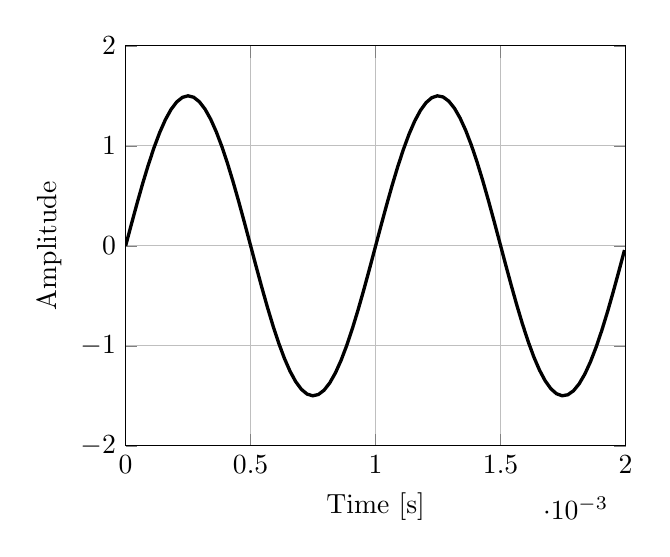
\begin{tikzpicture}

\begin{axis}[%
width=2.5in,
height=2in,
at={(1.011in,0.642in)},
scale only axis,
xmin=0,
xmax=0.002,
xlabel={Time [s]},
xmajorgrids,
ymin=-2,
ymax=2,
ylabel={Amplitude},
ymajorgrids,
axis background/.style={fill=white}
]
\addplot [color=black,solid,line width=1.2pt,forget plot]
  table[row sep=crcr]{%
0	0\\
2.26757369614512e-05	0.21299147693644\\
4.53514739229025e-05	0.421666669997482\\
6.80272108843537e-05	0.621796765035443\\
9.0702947845805e-05	0.809326114779272\\
0.000113378684807256	0.98045442674729\\
0.000136054421768707	1.13171377638122\\
0.000158730158730159	1.26003888472616\\
0.00018140589569161	1.36282923647545\\
0.000204081632653061	1.43800177955499\\
0.000226757369614512	1.48403313828686\\
0.000249433106575964	1.49999048468041\\
0.000272108843537415	1.48555044224226\\
0.000294784580498866	1.44100563921852\\
0.000317460317460317	1.36725877846751\\
0.000340136054421769	1.26580434413712\\
0.00036281179138322	1.13869831586227\\
0.000385487528344671	0.988516504225587\\
0.000408163265306122	0.818302351815823\\
0.000430839002267574	0.631505257698036\\
0.000453514739229025	0.431910675153779\\
0.000476190476190476	0.223563399264262\\
0.000498866213151927	0.0106855989178377\\
0.000521541950113379	-0.202408745672383\\
0.00054421768707483	-0.411401266012395\\
0.000566893424036281	-0.612056717299934\\
0.000589569160997732	-0.800308805890951\\
0.000612244897959184	-0.972342592961682\\
0.000634920634920635	-1.1246718044516\\
0.000657596371882086	-1.25420948059704\\
0.000680272108843537	-1.35833053333888\\
0.000702947845804989	-1.43492494387492\\
0.00072562358276644	-1.48244052230586\\
0.000748299319727891	-1.49991436284804\\
0.000770975056689342	-1.48699235717159\\
0.000793650793650794	-1.44393637042502\\
0.000816326530612245	-1.37161893452372\\
0.000839002267573696	-1.2715055662432\\
0.000861678004535147	-1.14562506844185\\
0.000884353741496599	-0.996528416260569\\
0.00090702947845805	-0.827237061472641\\
0.000929705215419501	-0.641181702599088\\
0.000952380952380952	-0.442132761616357\\
0.000975056689342404	-0.234123976149712\\
0.000997732426303855	-0.0213706555606557\\
0.00102040816326531	0.191815742526759\\
0.00104308390022676	0.401114984149397\\
0.00106575963718821	0.602285608781499\\
0.00108843537414966	0.791250882763146\\
0.00111111111111111	0.964181414529808\\
0.00113378684807256	1.11757275744087\\
0.00115646258503401	1.24831642758161\\
0.00117913832199546	1.35376289735891\\
0.00120181405895692	1.43177528832223\\
0.00122448979591837	1.48077267512167\\
0.00124716553287982	1.49976212304635\\
0.00126984126984127	1.48835880990026\\
0.00129251700680272	1.44679382444511\\
0.00131519274376417	1.37590948337396\\
0.00133786848072562	1.27714226171757\\
0.00136054421768707	1.15249368259969\\
0.00138321995464853	1.00448975626204\\
0.00140589569160998	0.836129790329203\\
0.00142857142857143	0.650825608676338\\
0.00145124716553288	0.452332410632626\\
0.00147392290249433	0.244672671662413\\
0.00149659863945578	0.0320546276809519\\
0.00151927437641723	-0.181213005075519\\
0.00154195011337868	-0.390808346418877\\
0.00156462585034014	-0.592483935346407\\
0.00158730158730159	-0.782152805069245\\
0.00160997732426304	-0.955971305616867\\
0.00163265306122449	-1.11041699561297\\
0.00165532879818594	-1.24236002474175\\
0.00167800453514739	-1.34912656033491\\
0.00170068027210884	-1.42855297273628\\
0.00172335600907029	-1.47902968137455\\
0.00174603174603175	-1.49953377300122\\
0.0017687074829932	-1.48964973108323\\
0.00179138321995465	-1.44957785626813\\
0.0018140589569161	-1.38013020728057\\
0.00183673469387755	-1.28271414450802\\
0.001859410430839	-1.15930380976591\\
0.00188208616780045	-1.01240012020625\\
0.0019047619047619	-0.844980087095434\\
0.00192743764172336	-0.660436486518814\\
0.00195011337868481	-0.462509104588652\\
0.00197278911564626	-0.25520895047495\\
0.00199546485260771	-0.0427369730862695\\
};
\end{axis}
\end{tikzpicture}%
%        \vspace{2mm}
%        \caption{Frequency response using impulse invariance method\citep{oppenheim}.}
%        \label{fig:impulse_invariance}
%    \end{subfigure} 
%    \hspace{4mm} 
%\begin{subfigure}[b]{0.48\textwidth}
%	\tikzsetnextfilename{clippingClean}
%	% This file was created by matlab2tikz.
%
%The latest updates can be retrieved from
%  http://www.mathworks.com/matlabcentral/fileexchange/22022-matlab2tikz-matlab2tikz
%where you can also make suggestions and rate matlab2tikz.
%
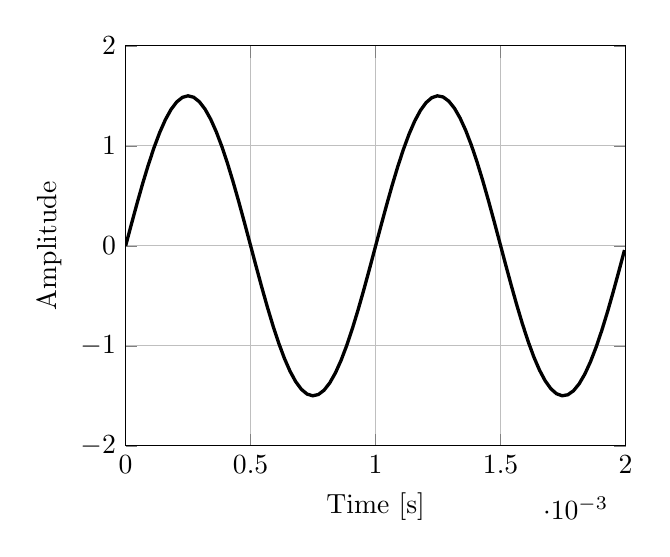
\begin{tikzpicture}

\begin{axis}[%
width=2.5in,
height=2in,
at={(1.011in,0.642in)},
scale only axis,
xmin=0,
xmax=0.002,
xlabel={Time [s]},
xmajorgrids,
ymin=-2,
ymax=2,
ylabel={Amplitude},
ymajorgrids,
axis background/.style={fill=white}
]
\addplot [color=black,solid,line width=1.2pt,forget plot]
  table[row sep=crcr]{%
0	0\\
2.26757369614512e-05	0.21299147693644\\
4.53514739229025e-05	0.421666669997482\\
6.80272108843537e-05	0.621796765035443\\
9.0702947845805e-05	0.809326114779272\\
0.000113378684807256	0.98045442674729\\
0.000136054421768707	1.13171377638122\\
0.000158730158730159	1.26003888472616\\
0.00018140589569161	1.36282923647545\\
0.000204081632653061	1.43800177955499\\
0.000226757369614512	1.48403313828686\\
0.000249433106575964	1.49999048468041\\
0.000272108843537415	1.48555044224226\\
0.000294784580498866	1.44100563921852\\
0.000317460317460317	1.36725877846751\\
0.000340136054421769	1.26580434413712\\
0.00036281179138322	1.13869831586227\\
0.000385487528344671	0.988516504225587\\
0.000408163265306122	0.818302351815823\\
0.000430839002267574	0.631505257698036\\
0.000453514739229025	0.431910675153779\\
0.000476190476190476	0.223563399264262\\
0.000498866213151927	0.0106855989178377\\
0.000521541950113379	-0.202408745672383\\
0.00054421768707483	-0.411401266012395\\
0.000566893424036281	-0.612056717299934\\
0.000589569160997732	-0.800308805890951\\
0.000612244897959184	-0.972342592961682\\
0.000634920634920635	-1.1246718044516\\
0.000657596371882086	-1.25420948059704\\
0.000680272108843537	-1.35833053333888\\
0.000702947845804989	-1.43492494387492\\
0.00072562358276644	-1.48244052230586\\
0.000748299319727891	-1.49991436284804\\
0.000770975056689342	-1.48699235717159\\
0.000793650793650794	-1.44393637042502\\
0.000816326530612245	-1.37161893452372\\
0.000839002267573696	-1.2715055662432\\
0.000861678004535147	-1.14562506844185\\
0.000884353741496599	-0.996528416260569\\
0.00090702947845805	-0.827237061472641\\
0.000929705215419501	-0.641181702599088\\
0.000952380952380952	-0.442132761616357\\
0.000975056689342404	-0.234123976149712\\
0.000997732426303855	-0.0213706555606557\\
0.00102040816326531	0.191815742526759\\
0.00104308390022676	0.401114984149397\\
0.00106575963718821	0.602285608781499\\
0.00108843537414966	0.791250882763146\\
0.00111111111111111	0.964181414529808\\
0.00113378684807256	1.11757275744087\\
0.00115646258503401	1.24831642758161\\
0.00117913832199546	1.35376289735891\\
0.00120181405895692	1.43177528832223\\
0.00122448979591837	1.48077267512167\\
0.00124716553287982	1.49976212304635\\
0.00126984126984127	1.48835880990026\\
0.00129251700680272	1.44679382444511\\
0.00131519274376417	1.37590948337396\\
0.00133786848072562	1.27714226171757\\
0.00136054421768707	1.15249368259969\\
0.00138321995464853	1.00448975626204\\
0.00140589569160998	0.836129790329203\\
0.00142857142857143	0.650825608676338\\
0.00145124716553288	0.452332410632626\\
0.00147392290249433	0.244672671662413\\
0.00149659863945578	0.0320546276809519\\
0.00151927437641723	-0.181213005075519\\
0.00154195011337868	-0.390808346418877\\
0.00156462585034014	-0.592483935346407\\
0.00158730158730159	-0.782152805069245\\
0.00160997732426304	-0.955971305616867\\
0.00163265306122449	-1.11041699561297\\
0.00165532879818594	-1.24236002474175\\
0.00167800453514739	-1.34912656033491\\
0.00170068027210884	-1.42855297273628\\
0.00172335600907029	-1.47902968137455\\
0.00174603174603175	-1.49953377300122\\
0.0017687074829932	-1.48964973108323\\
0.00179138321995465	-1.44957785626813\\
0.0018140589569161	-1.38013020728057\\
0.00183673469387755	-1.28271414450802\\
0.001859410430839	-1.15930380976591\\
0.00188208616780045	-1.01240012020625\\
0.0019047619047619	-0.844980087095434\\
0.00192743764172336	-0.660436486518814\\
0.00195011337868481	-0.462509104588652\\
0.00197278911564626	-0.25520895047495\\
0.00199546485260771	-0.0427369730862695\\
};
\end{axis}
\end{tikzpicture}%
%        \vspace{2mm}
%        \caption{Frequency response using bilinear transformation\citep{oppenheim}.}
%        \label{fig:bilinear_transform}
%    \end{subfigure}  
%\caption{Comparison between the impulse invariance method and bilinear transformation.}
%\label{fig:filter_design_methods}
%\end{figure}